% =====================================================================================
% SECTION 2: RESEARCH PROBLEM AND REQUIREMENTS  
% =====================================================================================

\section{Research Problem and Requirements}
\label{sec:problem}

\subsection{Problem Definition}
\label{subsec:problem_definition}

Our task requires solving three specific challenges for event type distribution visualization:

\textbf{Calculate Event Timing:} For each event type, determine when events occur relative to case start time. This means computing time differences between each event and the first event in its case.

\textbf{Statistical Sorting:} Sort event types based on different statistical parameters including minimum, maximum, mean, median, and quartiles. Users need to explore data from multiple statistical perspectives.

\textbf{Violin Chart Visualization:} Display results using violin charts that show both distribution shape and statistical summaries. Traditional charts fail to reveal the complex patterns in process timing data.

\subsection{Current Visualization Problems}
\label{subsec:current_problems}

Existing process mining tools struggle with event timing visualization:

\textbf{Case-Start Dominance:} Figure \ref{fig:case_start_problem} shows how events at time = 0 create massive spikes that hide all other patterns. In our Traffic Fines dataset, 28.7\% of events occur at case start, making the visualization useless.

\textbf{Extreme Skewness:} Most process datasets have 80-90\% of events clustered in early time periods. Traditional histograms and box plots cannot handle this distribution shape effectively.

\textbf{Statistical Limitations:} Current charts show either distribution shape OR statistical summaries, but not both. Process analysts need to see mean, median, and quartiles alongside the distribution shape.

\textbf{Cross-Domain Differences:} Healthcare processes happen in hours, government processes take months, and financial processes span weeks. No single visualization approach handles all these time scales.

\subsection{Requirements Analysis}
\label{subsec:requirements}

Based on our task specifications and the identified problems, we establish these requirements:

\textbf{R1 - Event Time Calculation:} System must calculate time since case start for each event relative to the first event in its case.

\textbf{R2 - Case-Start Filtering:} Remove events where time since case start equals zero to eliminate visualization noise while preserving meaningful timing data.

\textbf{R3 - Violin Chart Implementation:} Use violin charts as specified in our task, showing distribution shape with integrated box plots for statistical summaries.

\textbf{R4 - Interactive Statistical Sorting:} Provide sorting options for minimum, maximum, mean, median, Q1, Q3, and frequency as specified in the requirements.

\textbf{R5 - Multi-Dataset Support:} Handle different process domains with varying time scales and event frequencies.

\textbf{R6 - Time Transformation Options:} Support multiple time scaling methods (logarithmic, square root, raw time units) to handle different distribution characteristics.

\textbf{R7 - Performance Requirements:} Maintain interactive response times (less than 1 second) for datasets ranging from thousands to millions of events.

\begin{figure}[H]
\centering
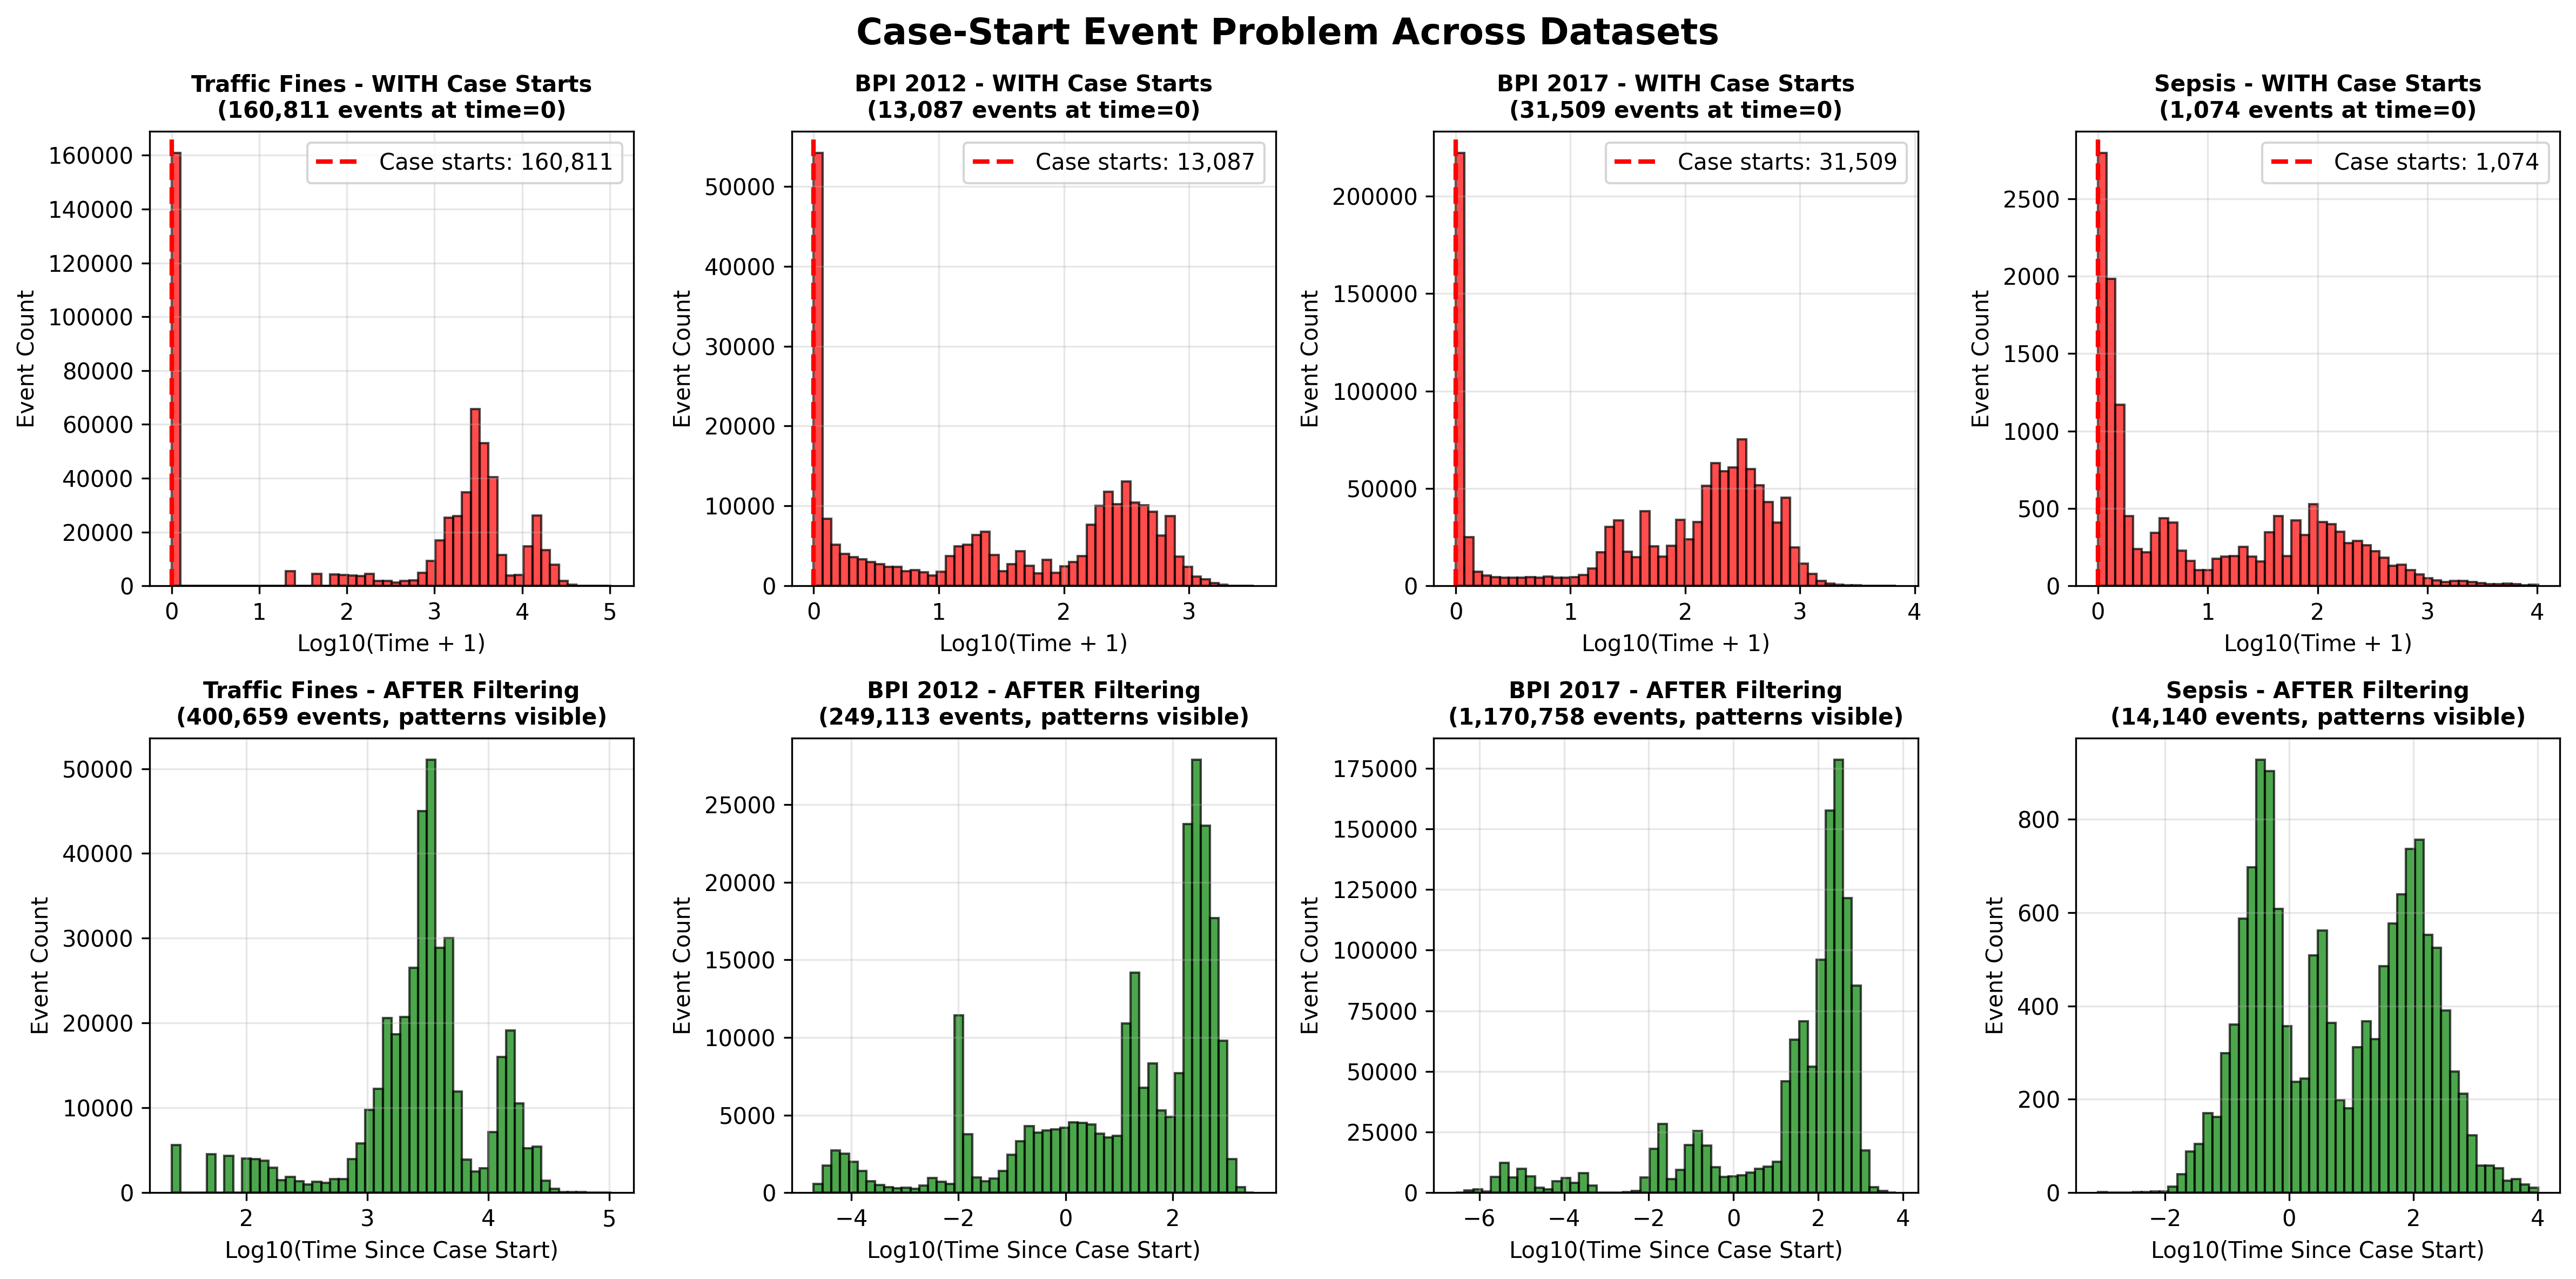
\includegraphics[width=\textwidth]{fig/case_start_problem.png}
\caption{Case-start event problem across four datasets. Top row shows traditional visualizations dominated by case-start events (red). Bottom row shows the same data after filtering, revealing meaningful timing patterns (green). Traffic Fines shows 28.6\% case-start events, BPI datasets show 2.6-5.0\%, and Sepsis shows 7.1\%.}
\label{fig:case_start_problem}
\end{figure}
